%Version 2.1 April 2023
% See section 11 of the User Manual for version history
%
%%%%%%%%%%%%%%%%%%%%%%%%%%%%%%%%%%%%%%%%%%%%%%%%%%%%%%%%%%%%%%%%%%%%%%
%%                                                                 %%
%% Please do not use \input{...} to include other tex files.       %%
%% Submit your LaTeX manuscript as one .tex document.              %%
%%                                                                 %%
%% All additional figures and files should be attached             %%
%% separately and not embedded in the \TeX\ document itself.       %%
%%                                                                 %%
%%%%%%%%%%%%%%%%%%%%%%%%%%%%%%%%%%%%%%%%%%%%%%%%%%%%%%%%%%%%%%%%%%%%%

\documentclass[sn-vancouver,Numbered,lineno,pdflatex]{sn-jnl}

%%%% Standard Packages
%%<additional latex packages if required can be included here>

\usepackage{graphicx}%
\usepackage{multirow}%
\usepackage{amsmath,amssymb,amsfonts}%
\usepackage{amsthm}%
\usepackage{mathrsfs}%
\usepackage[title]{appendix}%
\usepackage{xcolor}%
\usepackage{textcomp}%
\usepackage{manyfoot}%
\usepackage{booktabs}%
\usepackage{algorithm}%
\usepackage{algorithmicx}%
\usepackage{algpseudocode}%
\usepackage{listings}%
%%%%

%%%%%=============================================================================%%%%
%%%%  Remarks: This template is provided to aid authors with the preparation
%%%%  of original research articles intended for submission to journals published
%%%%  by Springer Nature. The guidance has been prepared in partnership with
%%%%  production teams to conform to Springer Nature technical requirements.
%%%%  Editorial and presentation requirements differ among journal portfolios and
%%%%  research disciplines. You may find sections in this template are irrelevant
%%%%  to your work and are empowered to omit any such section if allowed by the
%%%%  journal you intend to submit to. The submission guidelines and policies
%%%%  of the journal take precedence. A detailed User Manual is available in the
%%%%  template package for technical guidance.
%%%%%=============================================================================%%%%

\usepackage{natbib}
\usepackage{hyperref}
\usepackage[utf8]{inputenc}
\usepackage{capt-of}
\usepackage{booktabs}
\usepackage{amssymb}
\usepackage{threeparttable}
\usepackage{float}
%\floatplacement{figure}{H}
%\floatplacement{table}{H}
\usepackage{lipsum,caption}
\geometry{
  a4paper,
  left=1in,
  right=1in,
  top=1in,
  bottom=1in,
  includeheadfoot
}
\usepackage{setspace}
%\usepackage{lineno}
%\linenumbers
\usepackage{siunitx}
\sisetup{
  mode = match,
  propagate-math-font = true,
  reset-math-version = false,
  reset-text-family = false,
  reset-text-series = false,
  reset-text-shape = false,
  text-family-to-math = true,
  text-series-to-math = true
}
\doublespacing
% Disable explicit page breaks in LaTeX
\let\clearpage\relax



\raggedbottom




% tightlist command for lists without linebreak
\providecommand{\tightlist}{%
  \setlength{\itemsep}{0pt}\setlength{\parskip}{0pt}}





\begin{document}


\title[High-Dimensional Propensity Score]{Is There a Competitive
Advantage to Using Multivariate Statistical or Machine Learning Methods
Over the Bross Formula in the hdPS Framework for Bias and Variance
Estimation?}

%%=============================================================%%
%% Prefix	-> \pfx{Dr}
%% GivenName	-> \fnm{Joergen W.}
%% Particle	-> \spfx{van der} -> surname prefix
%% FamilyName	-> \sur{Ploeg}
%% Suffix	-> \sfx{IV}
%% NatureName	-> \tanm{Poet Laureate} -> Title after name
%% Degrees	-> \dgr{MSc, PhD}
%% \author*[1,2]{\pfx{Dr} \fnm{Joergen W.} \spfx{van der} \sur{Ploeg} \sfx{IV} \tanm{Poet Laureate}
%%                 \dgr{MSc, PhD}}\email{iauthor@gmail.com}
%%=============================================================%%

\author*[1,2]{\pfx{Dr.} \fnm{Mohammad Ehsanul} \sur{Karim} \dgr{MSc,
PhD}}\email{\href{mailto:ehsan.karim@ubc.ca}{\nolinkurl{ehsan.karim@ubc.ca}}}

\author[3]{\fnm{Yang} \sur{Lei} }



  \affil*[1]{\orgdiv{School of Population and Public
Health}, \orgname{University of British
Columbia}, \orgaddress{\city{Vancouver}, \country{Canada}, \postcode{V6T
1Z3}, \state{BC}, \street{2206 East Mall}}}
  \affil[2]{\orgname{St.~Paul's
Hospital}, \orgaddress{\city{Vancouver}, \country{Canada}, \postcode{V6Z
1Y6}, \state{BC}, \street{588 - 1081 Burrard Street}}}
  \affil[3]{\orgdiv{Department of Statistics}, \orgname{University of
British
Columbia}, \orgaddress{\city{Vancouver}, \country{Canada}, \postcode{V6T
1Z4}, \state{BC}, \street{Room 3182 Earth Sciences Building, 2207 Main
Mall}}}

\abstract{\textbf{Purpose}: We aim to evaluate various proxy selection
methods within the context of high-dimensional propensity score (hdPS)
analysis. This study aimed to systematically evaluate and compare the
performance of traditional statistical methods and machine learning
approaches within the hdPS framework, focusing on key metrics such as
bias, standard error (SE), and coverage, under various exposure and
outcome prevalence scenarios. \textbf{Methods:} We conducted a plasmode
simulation study using data from the National Health and Nutrition
Examination Survey (NHANES) cycles from 2013 to 2018. We compared
methods including the kitchen sink model, Bross-based hdPS, Hybrid hdPS,
LASSO, Elastic Net, Random Forest, XGBoost, and Genetic Algorithm (GA).
The performance of each method was assessed based on bias, MSE, coverage
probability, and SE estimation across three epidemiological scenarios:
frequent exposure and outcome, rare exposure and frequent outcome, and
frequent exposure and rare outcome. \textbf{Results:} XGBoost
consistently demonstrated strong performance in terms of MSE and
coverage, making it effective for scenarios prioritizing precision.
However, it exhibited higher bias, particularly in rare exposure
scenarios, suggesting it is less suited when minimizing bias is
critical. In contrast, GA showed significant limitations, with
consistently high bias and MSE, making it the least reliable method.
Bross-based hdPS, and Hybrid hdPS methods provided a balanced approach,
with low bias and moderate MSE, though coverage varied depending on the
scenario. Rare outcome scenarios generally resulted in lower MSE and
better precision, while rare exposure scenarios were associated with
higher bias and MSE. Notably, traditional statistical approaches such as
forward selection and backward elimination performed comparably to more
sophisticated machine learning methods in terms of bias and coverage,
suggesting that these simpler approaches may be viable alternatives due
to their computational efficiency. \textbf{Conclusion:} The results
highlight the importance of selecting hdPS methods based on the specific
characteristics of the data, such as exposure and outcome prevalence.
While advanced machine learning methods such as XGBoost can enhance
precision, simpler methods such as forward selection or backward
elimination may offer similar performance in terms of bias and coverage
with fewer computational demands. Tailoring the choice of method to the
epidemiological scenario is essential for optimizing the balance between
bias reduction and precision.}

\keywords{Machine learning, Propensity score, Deep learning, Causal
inference}


\pacs[JEL Classification]{C18}
\pacs[MSC Classification]{92D30, 62P10}

\maketitle

\section{Background}\label{background}

\textbf{High-dimensional Propensity Score (hdPS) Algorithm}: In
epidemiology, proxy variables are commonly used as substitutes for
confounders that are difficult or impossible to measure directly, such
as socioeconomic status, lifestyle factors, or health behaviors
\citep{vanderweele2019principles}. The hdPS is a pharmacoepidemiological
method designed to reduce confounding bias in large healthcare databases
\citep{schneeweiss2009high}. Unlike traditional propensity score models
that rely on investigator-specified or manually selected covariates,
hdPS automatically ranks a wide array of proxy variables from healthcare
records---such as diagnosis codes, medications, and procedures---using
the Bross formula \citep{wyss2018erratum, bross1966spurious}. The Bross
formula ranks these variables based on their marginal associations with
both exposure and outcome. These selected proxy variables serve as
surrogates for unmeasured or poorly measured confounders, helping reduce
bias in treatment effect estimates. The hdPS algorithm further refines
the selection by prioritizing variables based on their prevalence and
potential for confounding, defined by their association with both
exposure and outcome \citep{schneeweiss2009high}.

\textbf{Multivariate Machine Learning Extensions}: Although the Bross
formula performs well in certain contexts, it has limitations in
capturing complex interactions, nonlinearities, and higher-order
associations between variables, especially in high-dimensional settings
where it does not account for the multivariate structure of other
covariates \citep{karim2024high, karim2018can}. To address these
model-specification-related limitations, multivariate machine learning
methods such as LASSO, Elastic Net, and Random Forests have been applied
within the hdPS framework. These methods are better suited for
high-dimensional data, where they can more effectively handle complex
relationships and improve the selection of proxy variables, thus
enhancing the precision of treatment effect estimates
\citep{karim2018can, schneeweiss2017variable, franklin2015regularized}.
Simulation studies and empirical research have shown that these machine
learning-based methods, or hybrid approaches combining the Bross formula
with machine learning, can reduce confounding more effectively and
increase efficiency compared to the Bross formula alone in certain
settings
\citep{karim2018can, schneeweiss2017variable, franklin2015regularized}.

\textbf{Assessing the Simulation Performance}: Other than bias, previous
studies have primarily focused on Mean Squared Error (MSE) as a key
metric for evaluating the performance of hdPS and its machine learning
extensions
\citep{franklin2015regularized, pang2016effect, wyss2018using, karim2018can, simon2023evaluating}.
However, in high-dimensional settings with singly robust methods, such
as hdPS and machine learning approaches such as LASSO, MSE may not
always be the most reliable measure. MSE combines both bias and variance
into a single metric, which makes interpretation challenging when
variance estimation is unstable---a common issue in these methods. In
contrast, coverage, which measures the proportion of confidence
intervals that capture the true treatment effect, provides a more direct
and meaningful assessment of a model's reliability. In realistic
observational studies, where model misspecification is often inevitable,
coverage---along with related metrics such as bias-eliminated coverage
and relative error in standard error (SE; which compares model-based SE
with empirical SE)---can reveal whether confidence intervals or SEs are
too narrow (underestimating uncertainty) or too wide (overestimating
uncertainty). This insight is crucial in determining whether the model
delivers valid estimates despite misspecification. Even a model with
poor MSE but good coverage may still be valuable, as it produces
realistic confidence intervals. By shifting the focus to coverage,
rather than relying solely on MSE, we can achieve a more comprehensive
understanding of method performance, especially in cases where unstable
variance estimation might distort conclusions drawn from MSE alone.

\textbf{Aim}: This research aims to systematically evaluate and compare
various proxy selection methods within the hdPS framework, using a
diverse range of simulation performance metrics, including bias, MSE,
and coverage. The study focuses on assessing how these alternative
statistical and machine leartning methods perform in selecting proxy
variables for confounding adjustment, compared to the traditional Bross
formula.

\section{Methods}\label{methods}

\subsection*{Data and Simulation}\label{data-and-simulation}
\addcontentsline{toc}{subsection}{Data and Simulation}

\textbf{Motivating Example}: We revisited the association between
obesity and the risk of diabetes using data from three cycles of the
National Health and Nutrition Examination Survey (NHANES) covering the
years 2013-2014, 2015-2016, and 2017-2018 \citep{karim2024high}. To
identify relevant investigator-specified covariates, we constructed a
causal diagram based on literature
\citep{saydah2014trends, liu2013association, kabadi2012joint, ostchega2012abdominal}
and established causal inference principles \citep{greenland1999causal}.
The covariates included in our analysis were carefully selected and
categorized into demographic, behavioral, health history,
access-related, and laboratory variables. While most of these variables
were binary or categorical, the Laboratory variables were continuous.

\textbf{Plasmode simulation}: To rigorously assess the performance of
the methods under consideration, we employed a plasmode simulation
framework, which is particularly well-suited for reflecting real-world
data structures and complexities \citep{franklin2014plasmode}. This
approach was inspired by the analytic dataset derived from NHANES and
involved resampling from the observed covariates and exposure
information (i.e., obesity) without altering them. By mirroring key
aspects of an actual epidemiological study, this simulation framework
offers a substantial advantage over traditional Monte Carlo simulations,
which often rely on hypothetical assumptions.

\textbf{Simulation scenarios under consideration}: Our plasmode
simulation was conducted over 500 iterations. For the base simulation
scenario, we set the prevalence of exposure (obesity) and the event rate
(diabetes) at 30\%, with a true odds ratio (OR) parameter of 1,
corresponding to a risk difference (RD) of 0. Each simulated dataset had
a sample size of 3,000 participants. The description of other scenarios
under consideration is provided in Table \ref{table:scenarios}.

\begin{table}[ht]
\centering
\caption{Overview of Plasmode Simulation Scenarios Reflecting Varying Exposure and Outcome Prevalences Based on National Health and Nutrition Examination Survey (NHANES) Data Cycles (2013-2018)}
\label{table:scenarios}
\begin{tabular}{lcccc}
  \toprule
  \textbf{Plasmode Simulation Scenario} & \textbf{Exposure} & \textbf{Outcome} & \textbf{True} & \textbf{Sample}\\
  \textbf{} & \textbf{Prevalence} & \textbf{Prevalence} & \textbf{Odds Ratio} & \textbf{Size}\\
  \midrule
  (i) Frequent Exposure and Outcome (Base) & 30\% & 30\% & 1 & 3,000 \\
  (ii) Rare Exposure and Frequent Outcome & 5\% & 30\% & 1 & 3,000 \\
  (iii) Frequent Exposure and Rare Outcome & 30\% & 5\% & 1 & 3,000 \\
  \bottomrule
\end{tabular}
\end{table}

\textbf{True Data Generating Mechanism Used in Plasmode Simulation}: The
primary goal of this plasmode simulation study is to evaluate various
variable selection methods under realistic conditions. To achieve this,
we formulated the outcome data based on a specific model specification
that incorporates both exposure and covariates, including
investigator-specified and proxy variables. The model specification
consists of three key components (See Appendices \S A and B for further
details):

\begin{enumerate}
\def\labelenumi{\arabic{enumi}.}
\item
  \emph{Investigator-Specified Covariates}: We retained the original
  investigator-specified covariates, which were either binary or
  categorical, reflecting how real-world studies typically operate.
\item
  \emph{Transformation of Laboratory Variables}: In real-world studies,
  it is common for analysts to lack precise knowledge of the true model
  specification. To simulate this uncertainty, we transformed the
  continuous laboratory variables using complex functions such as
  logarithmic, exponential, square root, polynomial transformations, and
  interactions. This reflects the challenges analysts face in correctly
  specifying models when dealing with continuous data.
\item
  \emph{Inclusion of Proxy Variables}: Real-world studies often deal
  with unmeasured confounding, which researchers attempt to mitigate by
  adding proxy variables. However, when a large number of proxies are
  added, some may act as noise variables, contributing little or nothing
  to the analysis. To simulate this, we selected only those binary proxy
  covariates (referred to as recurrence covariates in hdPS terminology)
  that had a relative risk (RR) of less than 0.8 or greater than 1.2
  concerning the outcome. Out of 142 proxy covariates, 94 met this
  criterion and were included in calculating a simple comorbidity burden
  measure. The remaining 48 covariates were excluded from this
  calculation and considered noise. This comorbidity burden measure (one
  variable) was then incorporated into our model specification for
  generating the outcome data.
\end{enumerate}

\textbf{Performance Measures}: From this simulation, we derived several
performance metrics to evaluate the effectiveness of the methods under
consideration: (1) bias, (2) average model-based SE (the average of
estimated SEs obtained from a model over repeated samples), (3)
empirical SE (the standard deviation of estimated treatment effects
across repeated samples), (4) MSE, (5) coverage probability of 95\%
confidence intervals, (6) bias-corrected coverage, and (7) Zip plot
\citep{morris2019using, white2023check}.

\subsection*{Estimators under
consideration}\label{estimators-under-consideration}
\addcontentsline{toc}{subsection}{Estimators under consideration}

The comparison between the data generation process and the analysis
process reveals two key differences: (i) The data generation used
transformed laboratory variables, whereas the analysis was conducted
using only the original laboratory variables. (ii) The data generation
employed a simple sum of selected proxy variables (sum of 94 proxy
covariates), while the analysis included all proxy variables (142 binary
proxies), with 48 of these acting as noise variables. These differences
help us assess how the proxy variable selection methods handle model
misspecification and the presence of noise variables.

\begin{enumerate}
\def\labelenumi{\arabic{enumi}.}
\item
  \textbf{Kitchen sink model}: This is a base model for comparison,
  where no variable selection approaches were used. All
  investigator-selected features and all proxy variables were used to
  model \citep{karim2018can}.
\item
  \textbf{hdPS using Bross formula}: The Bross formula is a statistical
  method used to calculate the bias introduced by not adjusting for a
  covariate \citep{bross1966spurious}. In hdPS analysis, this formula
  was originally applied to each proxy variable to measure and rank the
  potential bias if the covariate were not adjusted for. In our
  analysis, the 100 proxies with the highest bias rankings are selected
  for further modeling \citep{schneeweiss2009high, wyss2018erratum}.
\item
  \textbf{Least Absolute Shrinkage and Selection Operator (LASSO)}:
  LASSO is a variable selection technique that limits the number of
  variables by adding a penalty term to the regression model.
  Cross-validation (CV) is used in LASSO to identify variables with
  non-zero coefficients in the best model by optimizing the penalty
  value
  \citep{franklin2015regularized, schneeweiss2017variable, karim2018can}.
\item
  \textbf{Hybrid of hdPS and LASSO}: Instead of relying solely on LASSO
  for variable selection, a hybrid approach combines the Bross formula
  and LASSO. First, proxy variables are selected using the hdPS
  algorithm (e.g., the top 100), and then LASSO is applied to further
  refine the selection \citep{karim2018can, franklin2015regularized}.
\item
  \textbf{Elastic Net}: Elastic Net is an extension of LASSO that
  includes an additional penalty term to handle multicollinearity by
  grouping correlated features and selecting the most representative
  ones \citep{karim2018can}.
\item
  \textbf{Random Forest}: The Random Forest algorithm is an ensemble
  learning method that constructs multiple decision trees to perform
  classification \citep{breiman2001random}. It calculates the importance
  of each proxy variable based on the decrease in impurity or Gini
  importance, providing a ranking of the proxies. The top 100 variables
  from this ranking are manually selected for further modeling
  \citep{schneeweiss2017variable}.
\item
  \textbf{XGBoost}: XGBoost is a gradient boosting algorithm used to
  optimize machine learning models \citep{chen2016xgboost}. It builds
  decision trees that make splits based on maximum impurity reduction,
  and it assigns an importance score to each proxy variable by
  calculating the mean decrease in impurity
  \citep{xiao2024interpretable}.
\item
  \textbf{Stepwise}: Stepwise selection is a progressive feature
  selection method that can proceed in two directions---forward or
  backward---based on the maximum adjusted R-squared. We have
  implemented two versions: (a) Forward selection (FS) starts with an
  initial model (e.g., including all investigator-selected features) and
  adds proxies to the model one at a time. (b) Backward elimination (BE)
  starts with a full model (e.g., all investigator-selected features and
  all proxy variables) and removes features one at a time based on their
  contribution to the model.
\item
  \textbf{Genetic algorithm}: Genetic algorithm is an evolutionary
  algorithm inspired by the theory of natural selection
  \citep{holland1975adaptation}. It operates by evolving offspring from
  a population of the fittest individuals over several generations,
  evaluating and selecting the best combination of features or variables
  that maximize prediction accuracy.
\end{enumerate}

\section{Results}\label{results}

The results for each method under the different scenarios are summarized
below. See Figures \ref{fig:bias-comparison} and
\ref{fig:Coverage-comparison} for an overview of the performance in
terms of bias and coverage, respectively. All simulation results can be
reviewed interactively through a Shiny web application available at
\url{https://ehsanx.shinyapps.io/hdPS-Alternatives/}, providing a
convenient platform for exploring the performance of each method across
various scenarios.

\begin{figure}[th]

{\centering 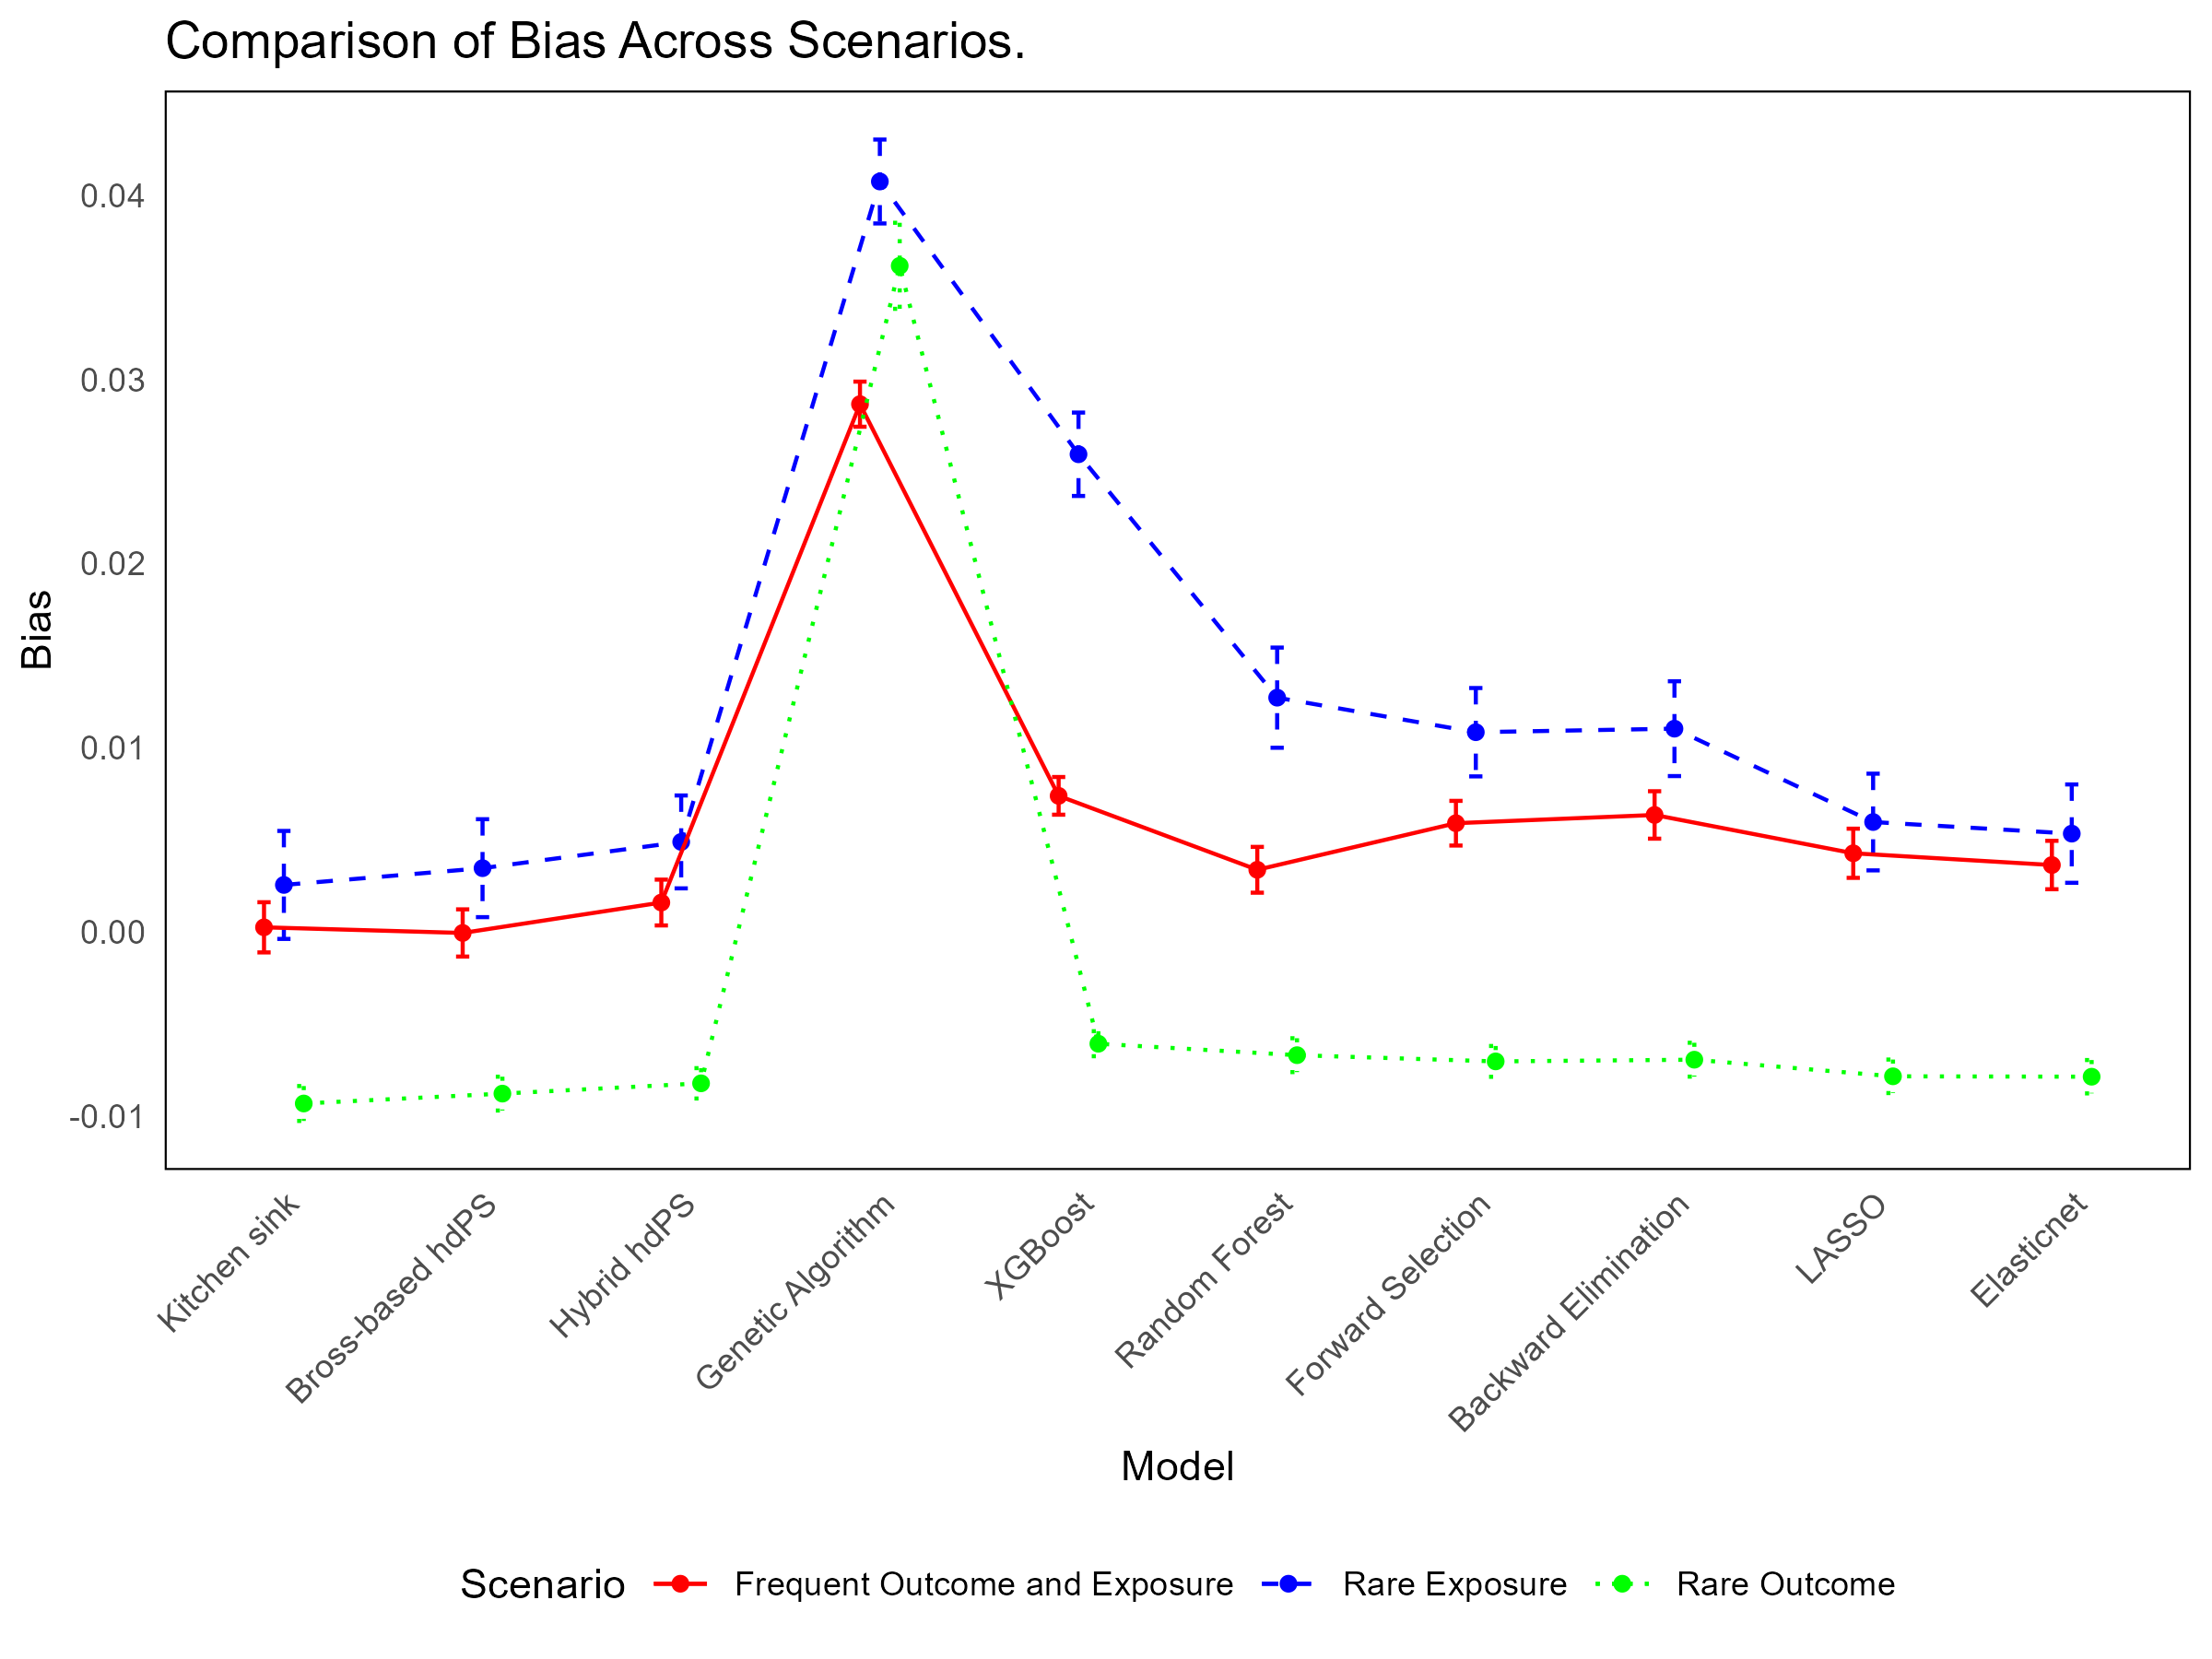
\includegraphics[width=1\linewidth,]{figures/metric_comparison_Bias} 

}

\caption{Comparison of Bias Across Different Methods in hdPS Analysis\label{fig:bias-comparison}}\label{fig:unnamed-chunk-1}
\end{figure}

\begin{figure}[th]

{\centering 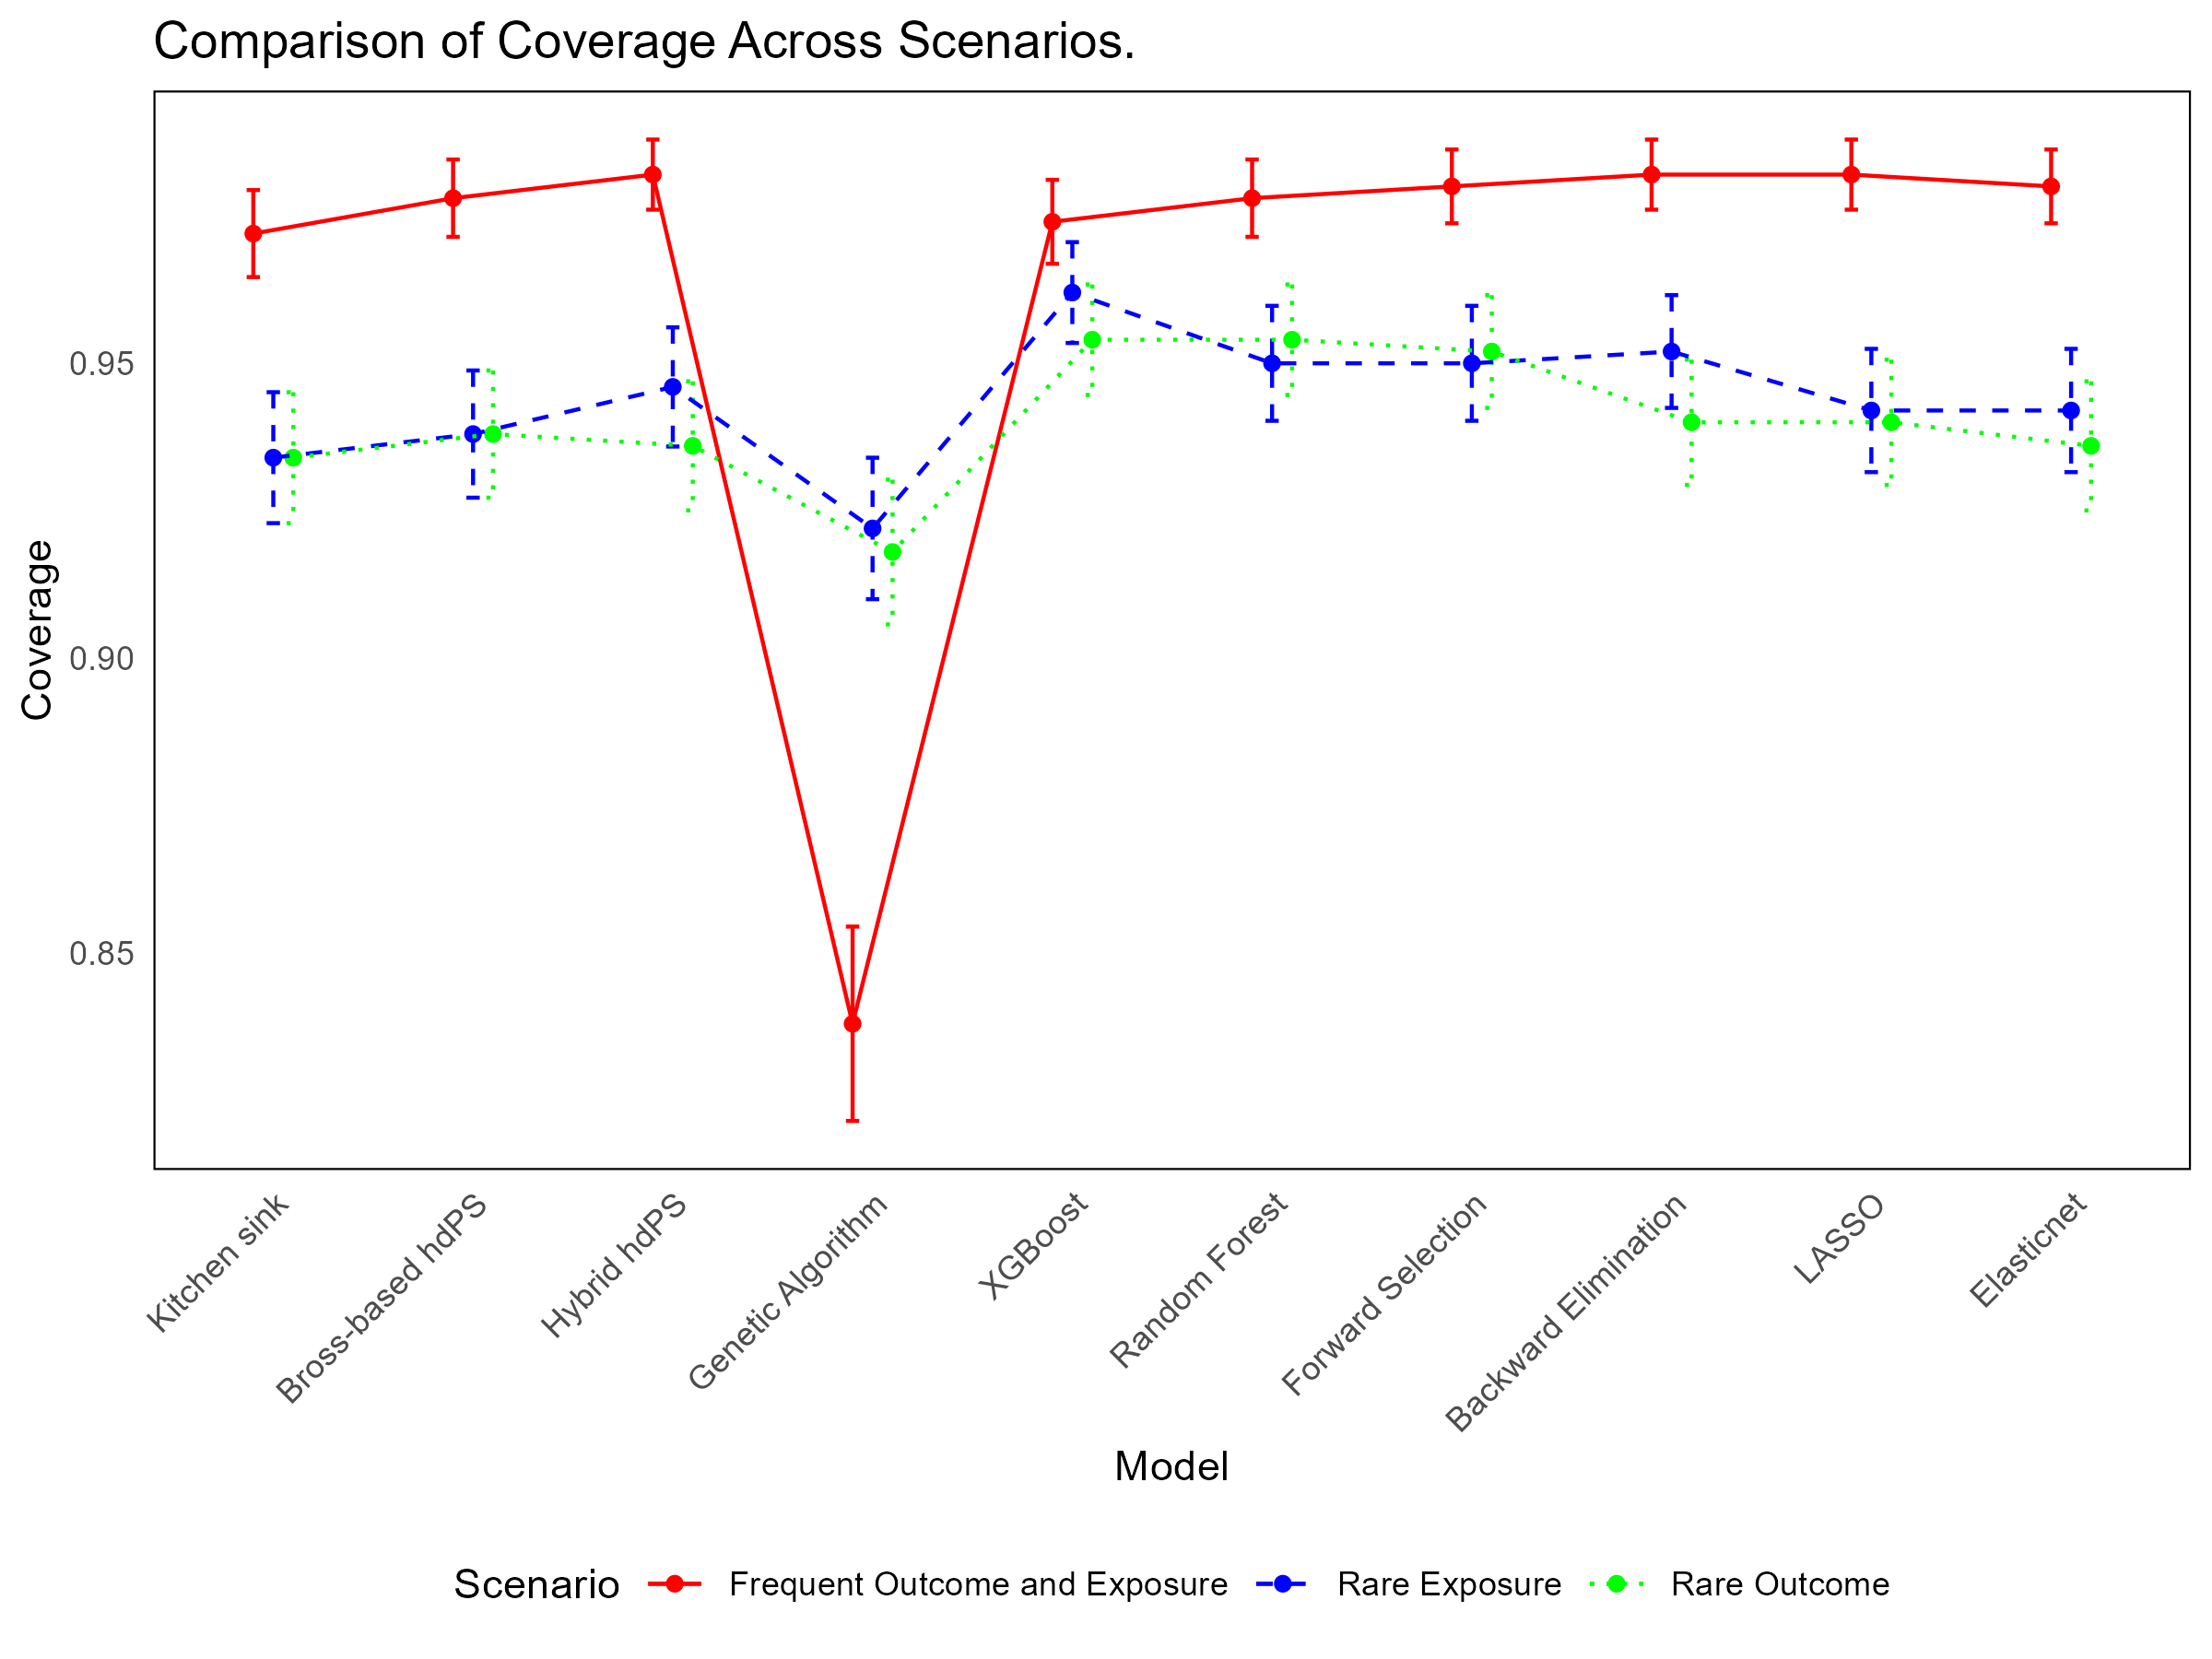
\includegraphics[width=1\linewidth,]{figures/metric_comparison_Coverage} 

}

\caption{Comparison of Coverage Probability Across Different Methods in hdPS Analysis\label{fig:Coverage-comparison}}\label{fig:unnamed-chunk-2}
\end{figure}

\begin{enumerate}
\def\labelenumi{(\roman{enumi})}
\tightlist
\item
  \textbf{Frequent Exposure and Outcome (base) scenario}:
\end{enumerate}

\begin{enumerate}
\def\labelenumi{\arabic{enumi}.}
\item
  \emph{Bias}: Bross-based hdPS exhibited the smallest bias (-0.0001),
  and the kitchen sink model (0.0002) was the second. Genetic algorithm
  shows the highest bias (0.0287), indicating a substantial deviation
  from the true effect. Among the other methods, Hybrid hdPS (0.0016),
  and Elastic Net (0.0036) demonstrated low bias. XGBoost (0.0074) had
  slightly higher bias than Random Forest (0.0034).
\item
  \emph{Coverage}: The coverage for most methods was high, with Hybrid
  hdPS, Forward Selection, Backward Elimination, LASSO, and Elastic Net
  achieving values around 98\%, indicating well-calibrated confidence
  intervals. However, Genetic algorithm had noticeably lower coverage
  (83.8\%), indicating that its confidence intervals might be too narrow
  or biased, potentially missing the true effect. After applying bias
  elimination (as there were substantial bias associated with this
  method), Genetic algorithm's coverage improved to 96\%.
\item
  \emph{MSE}: XGBoost achieved the lowest MSE (0.0006). Genetic
  algorithm maintained the highest MSE (0.0016), reflecting its higher
  bias and variability. The kitchen sink model (0.0009), Bross-based
  hdPS (0.0008), Hybrid hdPS (0.0008), and Elastic Net (0.0009) all had
  relatively similar and moderate MSE values.
\item
  \emph{SE}: XGBoost exhibited the lowest Empirical SE (0.0229),
  indicating high precision in its estimates. The kitchen sink model had
  the highest Empirical SE (0.0305), suggesting greater variability.
  Other methods, including Genetic algorithm (0.0274), Hybrid hdPS
  (0.0278), and Bross-based hdPS (0.0287), showed moderate variability.
  LASSO (0.0299) and Elastic Net (0.0294) had slightly higher
  variability. The Model-based SE followed a similar pattern, with
  XGBoost (0.0268) showing the lowest variability and the kitchen sink
  model (0.0333) the highest, indicating less precision in its
  estimates. When comparing relative error in SE estimation, XGBoost
  performed the worst. See Appendix \S C for further details.
\end{enumerate}

\textbf{(ii) Rare Exposure and Frequent Outcome}:

\begin{enumerate}
\def\labelenumi{\arabic{enumi}.}
\item
  \emph{Bias}: The kitchen sink model showed a relatively low bias
  (0.0025), while Genetic algorithm continued to exhibit the highest
  bias (0.0408), indicating a significant deviation from the true
  effect. XGBoost had a bias of 0.0259, which, while still higher than
  other methods, but was lower than Genetic algorithm. Other methods,
  such as Bross-based hdPS (0.0035), Hybrid hdPS (0.0049), and Elastic
  Net (0.0053), demonstrated moderate bias. Random Forest (0.0127) and
  Forward Selection (0.0108) had slightly higher bias but remained
  within an acceptable range.
\item
  \emph{Coverage}: Coverage levels remained high for most methods, with
  XGBoost achieving the highest coverage at 96.2\%, indicating
  well-calibrated confidence intervals despite its higher bias. The
  Genetic algorithm method had lower coverage (92.2\%), suggesting that
  its confidence intervals might be narrower, potentially missing the
  true effect. Other methods such as RF, Forward Selection, Backward
  Elimination, and Hybrid hdPS maintained coverage values around
  94-95\%, suggesting adequate interval calibration. Bias-eliminated
  coverage for Genetic algorithm improved to 94.2\%, but it was still
  slightly lower than other methods (e.g., forward selection).
\item
  \emph{MSE}: Forward selection demonstrated the lowest MSE (0.0030),
  and then Hybrid hdPS and XGBoost. The Genetic algorithm method had a
  higher MSE (0.0043), reflecting its substantial bias and variability.
  The kitchen sink model also had an MSE of 0.0043, similar to Genetic
  algorithm, while other methods such as Bross-based hdPS (0.0035), RF
  (0.0039), and Elastic Net (0.0036) exhibited moderate MSE values,
  indicating reasonable accuracy.
\item
  \emph{SE}: The lowest Empirical SE was observed with XGBoost (0.0507)
  and Genetic algorithm (0.0510), reflecting high precision despite
  their higher bias. The kitchen sink model had the highest Empirical SE
  (0.0656), indicating greater variability. Hybrid hdPS (0.0564),
  Bross-based hdPS (0.0595), and RF (0.0609) showed moderate
  variability. Forward Selection (0.0537) and Backward Elimination
  (0.0576) had lower variability compared to the kitchen sink model. In
  terms of Model-based SE, XGBoost (0.0531) and Genetic algorithm
  (0.0533) continued to show low variability, while the kitchen sink
  model had the highest Model-based SE (0.0623), indicating less
  precision in its estimates. When comparing relative error in SE
  estimation, XGBoost and kitchen sink model performed the worst (in
  other direction).
\end{enumerate}

\textbf{(iii) Frequent Exposure and Rare Outcome}:

\begin{enumerate}
\def\labelenumi{\arabic{enumi}.}
\item
  \emph{Bias}: In this scenario, the kitchen sink model exhibited a
  moderate negative bias (-0.0093), similar to the Bross-based hdPS
  method (-0.0088). Genetic algorithm showed a significantly higher bias
  (0.0362), indicating a substantial deviation from the true effect.
  Among other methods, XGBoost demonstrated the lowest bias (-0.0061),
  while methods such as Hybrid hdPS (-0.0082), Forward Selection
  (-0.0070), and Backward Elimination (-0.0070) had slightly higher but
  still moderate biases. Elastic Net and LASSO both had biases of
  -0.0079, reflecting slightly larger deviations compared to XGBoost but
  still within acceptable limits.
\item
  \emph{Coverage}: Most methods achieved good coverage, with XGBoost,
  RF, and Forward Selection each achieving a coverage rate of 95.4\%,
  indicating well-calibrated confidence intervals. The Genetic algorithm
  method, however, had slightly lower coverage (91.8\%), indicating that
  its confidence intervals might be narrower, potentially excluding the
  true effect. Bross-based hdPS and the kitchen sink model had slightly
  lower coverage values of 93.8\% and 93.4\%, respectively. After
  accounting for bias, the bias-eliminated coverage for most methods,
  except Genetic algorithm, remained high, with values ranging from
  98.4\% to 99.0\%, indicating that most methods effectively adjusted
  for bias in their coverage estimates. Genetic algorithm's
  bias-eliminated coverage was lower at 93.4\%, reflecting its higher
  inherent bias.
\item
  \emph{MSE}: XGBoost exhibited the lowest MSE (0.0003). Genetic
  algorithm had the highest MSE (0.0040), reflecting its substantial
  bias and variability. The kitchen sink model (0.0005), Bross-based
  hdPS (0.0005), and other methods such as Hybrid hdPS (0.0004) and
  Elastic Net (0.0005) all had relatively similar MSE values, indicating
  moderate accuracy.
\item
  \emph{SE}: The lowest Empirical SE was observed with XGBoost (0.0152),
  reflecting high precision in its estimates. The Genetic algorithm
  method exhibited the highest Empirical SE (0.0523), indicating greater
  variability and less precision. Methods such as Hybrid hdPS (0.0184),
  Forward Selection (0.0187), and Elastic Net (0.0203) showed moderate
  variability, while Bross-based hdPS (0.0206) and the kitchen sink
  model (0.0212) had slightly higher variability. In terms of
  Model-based SE, XGBoost (0.0179) again showed the lowest variability,
  consistent with its low Empirical SE, indicating that it provided the
  most stable estimates. The kitchen sink model had a slightly higher
  Model-based SE (0.0219), indicating less precision in its estimates.
  When comparing relative error in SE estimation, XGBoost performed the
  worst.
\end{enumerate}

\section{Real-world analysis}\label{real-world-analysis}

\textbf{Summary results}: The dataset comprises 7,585 individuals. Among
these, the prevalence of the exposure is 48.8\%, while the prevalence of
the outcome is 23.7\%.

See Figure \ref{fig:comparison-plot-updated} for the results from
analyzing the NHANES (2013-2018) dataset. The methods are arranged
according to the number of selected proxy variables. Among all variable
selection algorithms, Random Forest and XGBoost demonstrate the highest
ORs, with values of 1.59 and 1.56, respectively. The ORs for the
remaining methods cluster around 1.52. Additionally, with the exception
of RF and the Bross formula hdPS, a general pattern emerges where
methods selecting a larger number of proxy variables yield lower ORs.
For RD, RF and XGBoost also exhibit the highest value 0.08, while the
remaining methods converge around 0.077. The trend observed in the OR
results appears to persist in the RD analysis.

\begin{figure}[th]

{\centering 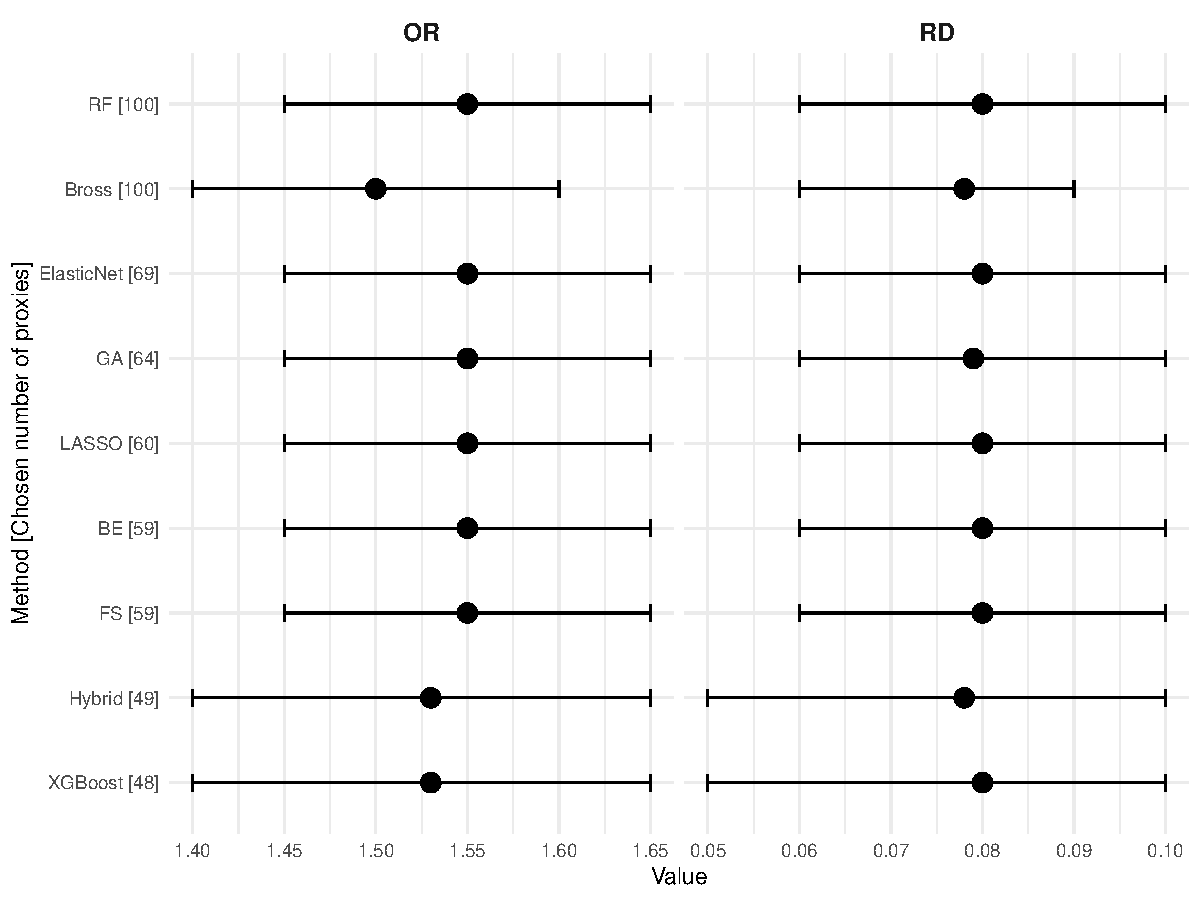
\includegraphics[width=1\linewidth,]{manuscript_files/figure-latex/unnamed-chunk-3-1} 

}

\caption{Figure presenting a comparison of Risk Differences (RD) and Odds Ratios (OR) with 95\% confidence intervals for different methods used to evaluate the association between obesity and diabetes risk. The analysis is based on data from the National Health and Nutrition Examination Survey (NHANES) for the years 2013-2018. Methods are arranged by the number of variables used in the models.\label{fig:comparison-plot-updated}}\label{fig:unnamed-chunk-3}
\end{figure}

Table \ref{tab:method-comparison-updated} presents a pairwise comparison
of the number of proxy features shared between different variable
selection methods used in the analysis. Each cell in the table indicates
the count of common proxy variables selected by the method in the
corresponding row and column. The diagonal cells, where the row and
column methods are the same, represent the total number of proxy
variables selected exclusively by each method. The first column displays
the number of proxy variables shared between each method and the kitchen
sink (KS) model. Given that the KS model includes all proxy variables,
the values in the first column are identical to those in the diagonal
cells for each row, which also presents the total number of proxy
variables selected by the method in the corresponding row.

\begin{table}[htbp]
\centering
\caption{Comparison of variable overlap of selected proxies across different methods used to evaluate the association between obesity and diabetes from the National Health and Nutrition Examination Survey (NHANES) for the years 2013-2018.}
\label{tab:method-comparison-updated}
\begin{tabular}{lcccccccccc}
\toprule
 & \textbf{KS} & \textbf{Bross} & \textbf{Hybrid} & \textbf{LASSO} & \textbf{EN} & \textbf{RF} & \textbf{XGB} & \textbf{FS} & \textbf{BE} & \textbf{GA} \\
\midrule
\textbf{Kitchen sink (KS)} & 142 & & & & & & & & & \\
\textbf{Bross formula} & 100 & 100 & & & & & & & & \\
\textbf{Hybrid (Bross and LASSO)} & 49 & 49 & 49 & & & & & & & \\
\textbf{LASSO} & 60 & 47 & 47 & 60 & & & & & & \\
\textbf{Elastic Net (EN)} & 69 & 54 & 48 & 60 & 69 & & & & & \\
\textbf{Random Forest (RF)} & 100 & 71 & 38 & 46 & 52 & 100 & & & & \\  
\textbf{XGBoost (XGB)} & 48 & 38 & 24 & 28 & 30 & 37 & 48 & & & \\
\textbf{Forward selection (FS)} & 59 & 45 & 41 & 51 & 54 & 45 & 25 & 59 & & \\
\textbf{Backward elimination (BE)} & 59 & 45 & 41 & 51 & 54 & 45 & 25 & 59 & 59 & \\
\textbf{Genetic algorithm (GA)} & 64 & 44 & 28 & 36 & 40 & 49 & 25 & 35 & 35 & 64 \\
\bottomrule
\end{tabular}
\end{table}

Table \ref{tab:proxy-common-pct-bross} presents a comparison of the
count and percentage of common proxy variables selected by different
methods in comparison with the Bross formula hdPS. The first column
shows the total number of proxy variables selected by each method, while
the second column lists the number of common features selected by both
the respective method and the Bross formula. The third column reports
the percentage of common features out of the total number of features
selected by each method.

We observe that, aside from the Bross formula hdPS and Random Forest
models, where the number of proxies was manually set to 100, and the
kitchen sink (KS) model, which includes all proxies by design, the
number of proxy variables selected by other models ranges between 49 and
69. As expected, the hybrid method combining Bross and LASSO hdPS
selects exactly 49 proxy variables, all of which are selected by both
methods, resulting in a common feature rate of 1.00. For other models,
the common feature percentage is generally clustered around \(74\%\),
with XGBoost showing the highest common percentage at \(79\%\), while
the Genetic Algorithm (GA) displays the lowest common percentage at
\(69\%\).

\begin{table}[htbp]
\centering
\caption{Comparison of the count and percentage of proxy variables selected by each methods in common with that by the Bross formula-based high-dimensional propensity score to evaluate the association between obesity and diabetes from the National Health and Nutrition Examination Survey (NHANES) for the years 2013-2018.}
\label{tab:proxy-common-pct-bross}
\begin{tabular}{lccc}
\toprule
\textbf{Method} & \textbf{Total Count} & \textbf{Common Count} & \textbf{Rate in Common} \\ 
\midrule
\textbf{Kitchen sink} & 142 & - & - \\
\textbf{Bross formula} & 100 & - & - \\
\textbf{Hybrid (Bross and LASSO)} & 49 & 49 & 1.00 \\
\textbf{LASSO} & 60 & 47 & 0.78 \\
\textbf{Elastic Net} & 69 & 54 & 0.78 \\
\textbf{Random Forest} & 100 & 71 & 0.71 \\  
\textbf{XGBoost} & 48 & 38 & 0.79 \\
\textbf{Forward selection} & 59 & 45 & 0.76 \\
\textbf{Backward elimination} & 59 & 45 & 0.76 \\
\textbf{Genetic algorithm} & 64 & 44 & 0.69 \\
\bottomrule
\end{tabular}
\end{table}

\textbf{Computing time}:

Figure \ref{fig:computing-time} presents the computing time for each
method. All methods, aside from RF and GA, exhibit relatively fast
computing times. RF and GA are generally much slower.

\begin{figure}[th]

{\centering 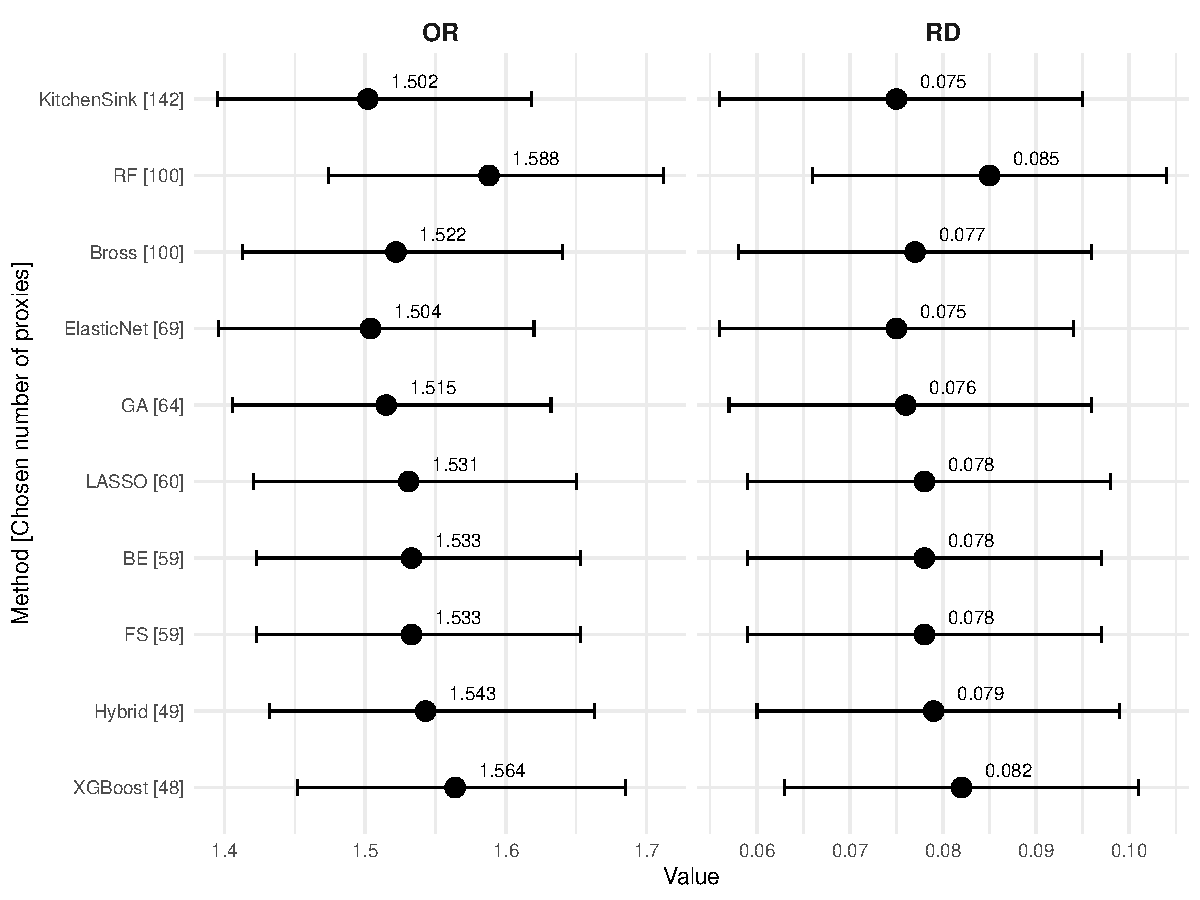
\includegraphics[width=1\linewidth,]{manuscript_files/figure-latex/unnamed-chunk-4-1} 

}

\caption{Computing time for the real-world analysis for each algorithm under consideration. The analysis is based on data from the National Health and Nutrition Examination Survey (NHANES) for the years 2013-2018.\label{fig:computing-time}}\label{fig:unnamed-chunk-4}
\end{figure}

\section{Discussion}\label{discussion}

\subsection{Summary of the simulation
findings}\label{summary-of-the-simulation-findings}

\textbf{Comparison of methods}:

Across the three scenarios, XGBoost consistently achieved the lowest MSE
and high coverage, making it one of the most reliable methods in terms
of precision. However, it consistently exhibited some degree of bias,
particularly when compared to methods such as the kitchen sink model,
Bross-based hdPS, and Hybrid hdPS, which often showed lower bias in
scenarios with frequent outcomes. In contrast, GA displayed the highest
bias and MSE, along with lower coverage and greater variability, making
it the least reliable method for accurate effect estimation. Methods
such as Bross-based hdPS, Hybrid hdPS, and Elastic Net performed
moderately well across all scenarios, balancing bias, coverage, and MSE.
However, these methods did not outperform XGBoost in terms of overall
precision, especially with respect to MSE, though they often resulted in
lower bias. The kitchen sink model performed comparably to Bross-based
hdPS in terms of bias and coverage but lagged in SE estimation and MSE.

\textbf{Comparison of scenarios}:

In scenarios with rare exposure, higher bias was observed, particularly
for methods such as GA and XGBoost, whereas frequent outcomes generally
led to lower bias across most methods. Overcoverage was more common in
the scenario with frequent exposure and outcome, with several methods
producing confidence intervals that were too wide, suggesting an
overestimation of uncertainty. The other scenarios exhibited more
balanced or slightly under-coverage. Scenarios with frequent exposure
also displayed higher relative error in SE estimation, making it more
difficult to precisely estimate effects. In contrast, rare exposure
scenarios were associated with higher MSE, reflecting the challenge of
estimating effects when the exposure is uncommon. Rare outcome scenarios
exhibited the lowest MSE across most methods (except GA), indicating
that these scenarios provided a better balance between bias and
precision for most methods.

\subsection{Contextualizing the
literature}\label{contextualizing-the-literature}

Previous studies have shown that LASSO performs well within the hdPS
framework, particularly in terms of bias reduction and MSE
\citep{karim2018can, franklin2015regularized}, with similar results for
Elastic Net \citep{karim2018can}. Our findings largely support these
conclusions, as both methods demonstrated moderate bias and MSE across
the scenarios. However, their performance was inconsistent in some
cases, with higher bias observed in rare exposure scenarios, as noted in
previous studies \citep{karim2018can, franklin2015regularized}. MSE also
increased in rare exposure scenarios. The Hybrid hdPS method, combining
Bross-based hdPS and LASSO, showed promising results, especially in
terms of MSE, suggesting it may serve as a suitable alternative to
traditional hdPS methods. Random Forest also performed similarly in our
study, yielding relatively low bias, which is consistent with previous
findings \citep{karim2018can}. However, none of the earlier works
emphasized coverage or examined methods such as GA, XGBoost, forward
selection, or backward elimination, which were evaluated here.

\subsection{Data analysis findings}\label{data-analysis-findings}

The real-world dataset, with frequent exposure (48.8\%) and a moderate
outcome rate (23.7\%), produced ORs of 1.59 and 1.56 for RF and XGBoost,
respectively, while other methods clustered around an OR of 1.52. A
general trend emerged, showing that methods selecting fewer proxy
variables yielded lower ORs, except for RF and the Bross formula hdPS.
In terms of risk difference (RD), estimates were relatively stable
across methods. Regarding variable overlap, most methods shared around
74\% of their proxy variables with the Bross formula hdPS, with XGBoost
showing the highest common rate (79\%) and GA the lowest (69\%).
Computing time analysis showed that, aside from RF and GA, most methods
had relatively fast computing times, with RF being significantly slower.

\subsection{Strengths}\label{strengths}

Previous studies on singly robust methods have mainly focused on hdPS
performance using MSE as the primary evaluation metric
\citep{franklin2015regularized, pang2016effect, wyss2018using, karim2018can, simon2023evaluating}.
Our study extends this body of work by incorporating a broader range of
performance metrics, allowing researchers to compare results in terms of
both bias and variance estimation. This comprehensive comparison of
statistical and machine learning methods across various scenarios has
not been conducted before. For instance, we found that while XGBoost
consistently demonstrated strong performance in terms of MSE and
coverage, it did not always have the lowest bias. Additionally, we
observed that traditional variable selection methods such as forward
selection and backward elimination performed similarly to more
sophisticated methods such as LASSO and Random Forest across scenarios,
both in terms of bias and coverage.

Our study also employed a complex plasmode simulation framework, closely
replicating real-world data conditions. This framework not only
accounted for model misspecification, where the true relationships
between covariates and outcomes were unknown, but also introduced noise
variables, addressing the challenge of dealing with irrelevant
covariates in high-dimensional settings. By applying transformations to
continuous variables and adding proxy variables that contributed
minimally to the outcome, we rigorously evaluated how well each method
handled both model uncertainty and non-informative variables, further
strengthening the real-world relevance of our findings.

\subsection{Future Direction}\label{future-direction}

Double robust methods have demonstrated strong potential for achieving
optimal statistical performance in hdPS analyses
\citep{pang2016targeted, pang2016effect, benasseur2022comparison}. In
addition, single robust methods, such as ensemble learners such as super
learners, have shown promise in improving bias, MSE, area under the
curve (AUC), and covariate balance in other contexts
\citep{guertin2016head, wyss2018using, ju2019propensity}. Deep learning
methods, particularly supervised architectures, offer significant
potential for improving propensity score estimation in high-dimensional
settings by capturing complex, non-linear relationships and performing
well in scenarios with rare exposures, while maintaining comparable bias
and superior variance estimation compared to traditional methods
\citep{karim2024can}. Despite their theoretical advantages, the
complexity and computational demands of these methods, especially in
high-dimensional settings, have limited their adoption by practitioners.
On the other hand, the simpler singly robust machine learning methods
evaluated here have been applied in clinical research
\citep{hossain2023role, basham2021post}.

Future research should explore the application of double robust methods
and super learners in hdPS analyses, particularly for handling rare
outcomes and exposures, where the performance of traditional methods may
be suboptimal. Additionally, investigating the impact of different
hyperparameters on machine learning methods such as XGBoost could
optimize their performance in hdPS analysis. Finally, future simulation
studies should focus on evaluating coverage and other metrics in
epidemiological scenarios such as time-varying exposures, which would
provide valuable insights into the generalizability of our findings
\citep{neugebauer2015high}.

\subsection{Conclusion}\label{conclusion}

In conclusion, this analysis highlights the importance of carefully
selecting appropriate methods for hdPS analysis based on the specific
characteristics of the data, particularly the prevalence of exposure and
outcome. These findings also emphasize the need to tailor method
selection to the specific epidemiological scenario, ensuring that the
chosen method aligns with the study's goals, whether minimizing bias or
maximizing precision.

XGBoost consistently demonstrated strong performance in terms of MSE and
coverage, making it an effective choice when precision is prioritized.
However, it did not achieve the lowest bias, particularly in rare
exposure scenarios, indicating that it may be less suited when
minimizing bias is the primary objective. In contrast, the Genetic
Algorithm (GA) exhibited significant limitations, with consistently high
bias and MSE, making it less reliable for effect estimation.

The kitchen sink, Bross-based hdPS, and Hybrid hdPS methods provided a
more balanced approach, offering low bias and moderate MSE, though
coverage varied depending on the scenario. The analysis also revealed
that rare outcomes were associated with lower MSE and better precision,
while rare exposures presented challenges, yielding higher bias and MSE.
Interestingly, traditional statistical approaches such as forward
selection and backward elimination performed comparably to more
sophisticated machine learning methods across many scenarios. This
suggests that simpler approaches can still be viable, particularly in
terms of bias and coverage, and might be preferred due to their
computational efficiency.

\section*{List of abbreviations}\label{list-of-abbreviations}
\addcontentsline{toc}{section}{List of abbreviations}

\begin{itemize}
\tightlist
\item
  hdPS: High-dimensional Propensity Score
\item
  NHANES: National Health and Nutrition Examination Survey
\item
  OR: Odds Ratio
\item
  RD: Risk Difference
\item
  SE: Standard Error
\item
  MSE: Mean Squared Error
\item
  KS: Kitchen Sink
\item
  LASSO: Least Absolute Shrinkage and Selection Operator
\item
  EN: Elastic Net; a regularized regression method that combines LASSO
  and Ridge regression
\item
  RF: Random Forest
\item
  XGBoost: Extreme Gradient Boosting
\item
  FS: Forward Selection
\item
  BE: Backward Elimination
\item
  GA: Genetic Algorithm
\item
  CV: Cross-Validation
\item
  RR: Relative Risk
\end{itemize}

\section*{Declarations}\label{declarations}
\addcontentsline{toc}{section}{Declarations}

\subsection*{Ethics approval and consent to
participate}\label{ethics-approval-and-consent-to-participate}
\addcontentsline{toc}{subsection}{Ethics approval and consent to
participate}

The analysis conducted on secondary and de-identified data is exempt
from research ethics approval requirements. Ethics for this study was
covered by item 7.10.3 in University of British Columbia's Policy \#89:
Research and Other Studies Involving Human Subjects 19 and Article 2.2
in of the Tri-Council Policy Statement: Ethical Conduct for Research
Involving Humans (TCPS2).

\subsection*{Consent for publication}\label{consent-for-publication}
\addcontentsline{toc}{subsection}{Consent for publication}

The National Health and Nutrition Examination Survey (NHANES), conducted
by the U.S. Centers for Disease Control and Prevention (CDC), involves
collecting data through direct physical examinations, laboratory
testing, and interviews. The CDC already obtains consent from
participants when collecting this data. When researchers use NHANES data
for their studies, they are typically using de-identified, publicly
available data. This means that the information cannot be linked back to
individual participants, and therefore, additional consent from
participants is not required for researchers to use this data.

\subsection*{Availability of data and
materials}\label{availability-of-data-and-materials}
\addcontentsline{toc}{subsection}{Availability of data and materials}

NHANES data is publicly accessible and can be retrieved from the NHANES
website. The datasets generated and/or analyzed during the current study
are available in the NHANES repository:
\url{https://www.cdc.gov/nchs/nhanes/index.htm}. Additionally, all
simulation results can be interactively reviewed through a Shiny web
application at \url{https://ehsanx.shinyapps.io/hdPS-Alternatives/}.

\subsection*{Clinical trial number}\label{clinical-trial-number}
\addcontentsline{toc}{subsection}{Clinical trial number}

Not applicable.

\subsection*{Competing interests}\label{competing-interests}
\addcontentsline{toc}{subsection}{Competing interests}

MEK is currently supported by grants from Canadian Institutes of Health
Research and MS Canada. MEK has previously received consulting fees from
Biogen Inc.~for consulting unrelated to this current work. MEK was also
previously supported by the Michael Smith Foundation for Health Research
Scholar award.

\subsection*{Funding}\label{funding}
\addcontentsline{toc}{subsection}{Funding}

This work was supported by MEK's Natural Sciences and Engineering
Research Council of Canada (NSERC) Discovery Grant (PG\#: 20R01603) and
Discovery Launch Supplement (PG\#: 20R12709).

\subsection*{Authors' contributions}\label{authors-contributions}
\addcontentsline{toc}{subsection}{Authors' contributions}

MEK: Conceptualization, Writing -- Original Draft, Review \& Editing YL:
Formal Analysis, Review \& Editing

\subsection*{Acknowledgements}\label{acknowledgements}
\addcontentsline{toc}{subsection}{Acknowledgements}

Not applicable.

\renewcommand\refname{References}
\bibliography{mergedbibliography.bib}


\end{document}
